% !TeX root = ./0-handout.tex

%details on counters; setting it to 0 prints everything with a roman I
%https://www.overleaf.com/learn/latex/Counters

%https://tex.stackexchange.com/questions/555149/how-do-i-change-the-frame-continuation-counter-from-roman-numerals-i-ii-iii

%\newcounter{mysection}
%\setcounter{mysection}{1}
%\arabic{mysection}
%\roman{subsection}

%\begin{itemize}[<+->] 
%\item<2-> % reveals second and keeps on page in subsequent frames
%\begin{itemize}[<2->] %does for a whole list of items


\setcounter{section}{-1} %sets section counter to 0. note that need to switch section counter from Roman to arabic for this to work! since no roman numeral for 0! %put this into preamble, i.e. file common.tex: \renewcommand\thesection{\arabic{section}}


\section{What is logic?}
%\subsection*{test}


%\subsection{But first: What is this class?}

%\iffalse
\begin{frame}
  \frametitle{But first: What is this class?}
  
  See the syllabus!!! See Canvas page! Enroll in \emph{Carnap} page!
  
    \begin{itemize}[<+->] 
        \item Download textbook: \textit{forallX Fall 2022 MIT edition} \\ (updated throughout semester, but hopefully not too drastically!)
    \item Problem Sets typically due Fridays 5pm
   \item Most problem sets submitted online via \emph{Carnap}
    \item Office hours could change based on when various reading groups are scheduled
    \item Located on 9th floor, Dreyfoos Wing; \\ turn RIGHT after entering Phil dept
    
  \end{itemize}

  
  \end{frame}

\frame{\frametitle{And second: Why come to class?}
\large
\begin{itemize}[<+->] 

\item We'll cover the essential content, in a digestible manner \\ (helpful if you find it hard to make time to read)

\item We'll do practice problems! Often geared toward homework and exam questions

\item You might gain some `insider information'

\bigskip

\item This is a \emph{skills-based} course: \\ the goal is to learn how to \emph{do} logic, rather than to memorize or regurgitate facts about logic.

\item Doing ample practice problems will be \emph{essential}!



\end{itemize}
}
  
  %\fi
  
  \begin{frame}
  \frametitle{Names and Quick Intros}
  
    \begin{itemize}[<+->]
    \item Ideally you'll feel completely comfortable in this class
    \item It'll probably be easier to focus if you feel comfortable
    \item I find it helps to say some words to feel comfortable!
    \item Let's say some words! 
    
  \end{itemize}
  
  \end{frame}


\subsection{Arguments and validity}

\frame{\frametitle{Causes vs. (normative) Reasons for belief}
\large
\begin{itemize}

\item \emph{Causes of belief}: why you actually believe something

\begin{itemize}[<2->]

\item Attacked by cat at age 8: causes you to believe `cats are dangerous'

\item These are \textit{descriptive} reasons for belief

\item Often these are not rationally compelling reasons

\end{itemize} 

\item<3->  \emph{Reasons for belief}: why you \textit{ought} to believe something

\begin{itemize}[<4->]

\item Empirical data on cat attacks per capita  

\item These are \textit{normative} reasons for belief

\item Logic aims to characterize the structure of such reasons, when organized into \textit{arguments}
% Tappenden: arguments are premises supporting conclusions that logically purport to give reasons for belief (not in the sense of causes for belief)

\end{itemize}

\end{itemize}
}

\frame{\frametitle{Rhetorically vs. Logically Good Arguments}
\large
\begin{itemize}

\item \emph{Rhetorically good argument}: argument that actually persuades listeners

\begin{itemize}[<2->]

\item Might be \textit{descriptively good}, while being logically awful

\item Might rely solely on emotional tricks or rhetoric

\item Anecdotes: ``my friend got a blood clot from the Johnson \& Johnson Covid vaccine. Therefore, avoid this vaccine!''  

\item A plane recently crashed: I better drive!

\end{itemize}

\item<3->  \emph{Logically good arguments}: arguments that \textit{ought} to persuade listeners, if they were rational

\begin{itemize}[<4->]

\item Such arguments might be descriptively pretty unpersuasive!

\item Comparative analysis of risk of blood clots from Janssen vaccine vs. risk of negative Covid health outcome 

\item Comparative analysis of plane crashes vs. car crashes

\end{itemize}



\end{itemize}
}

\begin{frame}
  \frametitle{An easy puzzle}

  \begin{block}{Where does Sanjeev live?}
  Sanjeev lives in Chicago or in Erie.\\
  Sanjeev doesn't live in Erie.
  \end{block}

  \begin{itemize}
    \item<2>[A:] Obviously, in Chicago.
  \end{itemize}

\end{frame}

\begin{frame}
  \frametitle{Arguments and sentences}

  \begin{block}{Argument 1}
  Sanjeev lives in Chicago or in Erie.\\
  Sanjeev doesn't live in Erie.\\
  Therefore, Sanjeev lives in Chicago.
  \end{block}

  \begin{itemize}[<+->]
  \item Such an argument consists of (declarative) \emph{sentences}.
  \item Declarative sentences are the kinds that can be \emph{true} or \emph{false}.
  \item ``Therefore'' ($\therefore$) indicates that the last sentence (supposedly)
  \emph{follows from} the first two.
  \item The last sentence is called the \emph{conclusion}.
  \item The others are called the \emph{premises}.
  \end{itemize}

\end{frame}

%JRH: would be better to contrest MP with affirming the consequent; e.g. Angela Merkel example 

\begin{frame}
  \frametitle{Valid and invalid arguments}

  \begin{block}{Argument 2}
  Mandy enjoys skiing or hiking (or both).\\
  Mandy doesn't enjoy hiking.\\
  $\therefore$ Mandy enjoys skiing.
  \end{block}

  \begin{block}{Argument 3}
  Mandy enjoys skiing or hiking (or both).\\
  Mandy enjoys skiing.\\
  $\therefore$ Mandy doesn't enjoy hiking.
  \end{block}

  What's the difference?

  \note[itemize]{
    \begin{itemize}
    \item Arg 2 is like argument 1
    \item Think-pair-share argument 2
    \item Depending on result of experiment/agreement talk about
    inclusive/exclusive
    \item Argument 2 is valid if the ``or'' is exclusive.
    \end{itemize}
  }
\end{frame}


\begin{frame}
  \frametitle{(Deductive) Validity}

  \begin{definition}<1->
  An argument is (deductively) \emph{valid} if there is no case where all its
  premises are true and the conclusion is false.
  \end{definition}

  \begin{definition}<2->
  An argument is \emph{invalid} if there is at least one case where
  all its premises are true and the conclusion is false (i.e., if it
  is not valid).
  \end{definition}

  \begin{definition}<3->
  A \emph{case} is some hypothetical scenario that makes each sentence
  in an argument either true or false.
  \end{definition}
\end{frame}

\begin{frame}
  \frametitle{Argument 2 is valid}

  \begin{block}{Argument 2}
  Mandy enjoys skiing or hiking.\\
  Mandy doesn't enjoy hiking.\\
  $\therefore$ Mandy enjoys skiing.
  \end{block}

Argument 2 is \emph{valid}: whenever the premises are
true, the conclusion is also true.

\end{frame}

\begin{frame}
  \frametitle{Argument 3 is not valid}

  \begin{block}{Argument 3}
  Mandy enjoys skiing or hiking.\\
  Mandy enjoys skiing.\\
  $\therefore$ Mandy doesn't enjoy hiking.
  \end{block}

  Argument 3 is \emph{invalid}: there is a possible case where the
  premises are true and the conclusion isn't (Mandy enjoys both skiing
  and hiking).

\end{frame}

\begin{frame}
  \frametitle{A harder puzzle}

  \begin{block}{Where does Sarah live?}
  Sarah lives in Chicago or Erie.\\
  Amir lives in Chicago unless he enjoys hiking.\\
  If Amir lives in Chicago, Sarah doesn't.\\
  Neither Sarah nor Amir enjoy hiking.
  \end{block}

\end{frame}

\subsection{Cases and determining validity}

\begin{frame}
  \frametitle{Validity}

  \begin{definition}
  An argument is \emph{valid} if there is no case where all its
  premises are true and the conclusion is false.
  \end{definition}

  \begin{definition}
  An argument is \emph{invalid} if there is at least one case where
  all its premises are true and the conclusion is false (i.e., if it
  is not valid).
  \end{definition}
\end{frame}

\begin{frame}{Cases}
  
\begin{definition}
  A \emph{case} is some hypothetical scenario that makes each sentence
  in an argument either true or false.
\end{definition}

\begin{itemize}[<+->]
  \item E.g., imagine you have a friend, her name is Mandy, she loves
  hiking but hates skiing.
  \item That's a case where ``Mandy enjoys hiking or skiing'' is true.
  \item Some cases can be imagined even though they never happen IRL, e.g,
  ``It is raining and the skies are clear.''
  \item Some things you can't imagine, e.g.,
  ``There is a blizzard but there is no wind.''
\end{itemize}

\end{frame}

\begin{frame}
  \frametitle{Determining validity}

  \begin{itemize}[<+->]
    \item Imagine a case where the conclusion is false.
    \item Are the premises true? You're done: invalid.
    \item Otherwise, change or expand the case to make them true
    (without making the conclusion also true).
    \item Can't? (Probably) valid.
  \end{itemize}

  \uncover<5->{OR}

  \begin{itemize}[<+->]
    \item Imagine a case where all premises are true.
    \item Is the conclusion false? You're done: invalid.
    \item Otherwise, change or expand the case to make it false
    (without making the premises false).
    \item Can't? (Probably) valid.
  \end{itemize}
\end{frame}

\begin{frame}{Deductively Valid?}
  \begin{earg}
    \item[] Some rodents have bushy tails.
    \item[] All squirrels are rodents.
    \item[\therefore] Some squirrels have bushy tails.
  \end{earg}
\pause
  \begin{itemize}[<+->]
    \item Imagine squirrels evolving so that they no longer have bushy
    tails. Then conclusion is false.
    \item But premises still true:
    \begin{itemize}[<+->]
      \item Imagine chinchillas still have bushy tails.
      \item Imagine also that squirrels have not evolved too
      much---they are still rodents.
    \end{itemize}
  \end{itemize}
\end{frame}

\begin{frame}{Valid?}
  \begin{earg}
    \item[] All rodents have bushy tails.
    \item[] All squirrels are rodents.
    \item[\therefore] All squirrels have bushy tails.
  \end{earg}
\pause
  \begin{itemize}[<+->]
    \item If it were invalid, you'd have a case that makes the
    conclusion false: some squirrels without bushy tails.
    \item They would have to be rodents still (otherwise premise 2 false).
    \item And that would require that they have bushy tails (otherwise premise 1 false).
  \end{itemize}
\end{frame}

\subsection{Other logical notions}

\begin{frame}
  \frametitle{Logical Consistency}

  \begin{definition}
  Sentences are (logically) \emph{consistent} if there is a case where they
  are all true. \\ $\bullet$ also called `jointly possible' or `satisfiable' 
  \end{definition}

  \begin{definition}
    Sentences are (logically) \emph{inconsistent} if there is no case where they
    are all true. \\ $\bullet$ also called `jointly impossible' or `unsatisfiable' 
    \end{definition}
\end{frame}


\begin{frame}
  \frametitle{Consistent?}
  \begin{earg}
    \item[] Some carnivores have bushy tails.
    \item[] All carnivores are mammals. 
    \item[] No mammals have bushy tails.
  \end{earg}

  \begin{itemize}
    \item<2> No case makes them all true at the same time, so
    \emph{inconsistent}.
  \end{itemize}
\end{frame}

\begin{frame}
  \frametitle{Valid?}
  \begin{earg}
    \item[] Some carnivores have bushy tails.
    \item[] All carnivores are mammals. 
    \item[] No mammals have bushy tails.
    \item[\therefore] All birds are carnivores. 
  \end{earg}

  \pause

  \begin{itemize}[<+->]
    \item The premises cannot all be true in the same case, so inconsistent.
    \item So: no case makes all the premises true.
    \item So also: no case makes the premises true and the conclusion false.
    \item \emph{Arguments with inconsistent premises are automatically
    valid}, regardless of what the conclusion is.
  \end{itemize}
\end{frame}

\begin{frame}{Tautology (logically necessary)}

  \begin{definition}
    A sentence is a \emph{tautology} if there is no case where
    it is false. \\ $\bullet$ also called a `necessary truth' or `truth-functionally true'
    \end{definition}
\pause
    \begin{itemize}[<+->]
      \item If it's snowing, then it's snowing.
      \item Every fawn is a deer.
      \item The number 5 is prime.
\item It's not the case that I am standing and that I am not standing. \\ (`\textit{Law of Non-Contradiction}')
      %\item Physical objects are extended.
    \end{itemize}
\end{frame}

\begin{frame}{Tautology}
    What can you say about an argument where the conclusion is a
    tautology? 
\pause
\begin{itemize}[<+->]
  \item If the conclusion is a tautology, there is no case where
  it is false.
  \item So there is no case where both (1) it is false and (2) the premises of the
  argument are all true.
  \item $\Rightarrow$ \emph{Arguments with tautologies as conclusions are
  automatically valid}, regardless of what the premises are.
\end{itemize}
  \end{frame}

\begin{frame}
  \frametitle{Logical equivalence}

  \begin{definition}
  Two sentences are (logically) \emph{equivalent} if there is no case where one is
  true and the other is false.
  \end{definition}

  \begin{itemize}[<+->]
    \item What can you say about an argument where one of the premises
    is equivalent to the conclusion? Is it automatically valid?
    \item Can you have two equivalent sentences that are inconsistent?
  \end{itemize}

\end{frame}


\subsection{What are we going to learn? \\ And why?}

\begin{frame}
  \frametitle{What is logic?}

  \begin{itemize}[<+->]
  \item \emph{Logic is the science of what follows from what.}
  \item Sometimes a conclusion follows from the premises, sometimes it
  does not:
  \begin{itemize}[<+->]
    \item Mandy lives in Chicago.\\ Everyone who lives in Chicago likes hiking.\\
    $\therefore$ Mandy likes hiking.
    \item Mandy lives in Chicago.\\ Everyone who likes hiking lives in Chicago.\\
    $\therefore$ Mandy likes hiking.
    \end{itemize}
  \item Logic investigates what makes the first argument \emph{valid}
    and the second \emph{invalid}.
  \end{itemize}
\end{frame}

\begin{frame}
  \frametitle{What is formal logic?}

  \begin{itemize}[<+->]
  \item Studies logical properties of \emph{formal languages} (SL and
  QL, not English).
    \begin{itemize}[<+->]
    \item Logical consequence (what follows from what?)
    \item Logical consistency (when do sentences contradict one another?)
    \end{itemize}
  \item Expressive power (what can be expressed in a given formal
  language, and how?)
  \item Formal models (mathematical structures described by formal language)
  \item Inference and proof systems (how can it be proved that something
  follows from something else?)
  \item Meta-logical properties of logical systems
  \end{itemize}
\end{frame}

\begin{frame}
  \frametitle{Plan for the course}

  \begin{itemize}[<+->]
  \item Sentential Logic (SL), aka Truth-functional logic
    \begin{itemize}[<+->]
    \item Symbolization in the formal language of SL ($H, \lor,
    \land, \to, \lnot$)
    \item Testing for validity: truth-tables and TREES! 
    \item Proofs in natural deduction
    \end{itemize}
  \item Quantifier Logic (QL), aka First-order logic 
    \begin{itemize}[<+->]
    \item More fine-grained symbolization ($E(m,h)$, $\forall$
    `every', $\exists$ `some', $=$)
    \item Semantics: interpretations
    \item Proofs in natural deduction
    \end{itemize}
  \item Metalogic (sprinkled in Unit 1 as well!): 
 \begin{itemize}[<+->]
\item Soundness \& Completeness of our deduction systems
\item Compactness
\item Expressive completeness, normal forms
  \end{itemize}
  \end{itemize}
\end{frame}

\begin{frame}
  \frametitle{What is logic good for? (Philosophy)}

  \begin{itemize}[<+->]
  \item Logic originates in philosophy (e.g. Aristotle); \\ traditionally considered a sub-discipline of philosophy.
  \item Valid arguments are critical in philosophical research.
  \item Formal tools of logic are useful for making various philosophical
  notions precise, e.g.,
    \begin{itemize}[<+->]
    \item Possibility and necessity
    \item Time
    \item Composition and parthood (mereology)
    \item Moral obligation and permissibility
    \item Belief and knowledge
    \end{itemize}
  \item Logic applies to the semantics of natural language \\ (philosophy of
  language, linguistics).
  \end{itemize}
\end{frame}

\begin{frame}
  \frametitle{What is logic good for? (Mathematics)}

  \begin{itemize}[<+->]
  \item Formal logic was developed largely in a quest for the foundations of
  mathematics (19th century).
  \item Logical systems provide precise foundational framework for
  mathematics:
    \begin{itemize}[<+->]
    \item Axiomatic systems (e.g, geometry)
    \item Algebraic structures (e.g., groups)
    \item Set theory (e.g, Zermelo-Fraenkel with Choice)
    \end{itemize}
  \item Precision
    \begin{itemize}[<+->]
    \item Formal language makes claims more precise.
    \item Formal structures can point to alternatives, unveil gaps in proofs.
    \item Formal proof systems make proofs rigorous.
    \item Formal proofs make mechanical \emph{proof checking} and \emph{proof search} possible.
    \end{itemize}
  \end{itemize}

\end{frame}


\begin{frame}
  \frametitle{What is logic good for? (Computer Science)}

  \begin{itemize}[<+->]
    \item Computer science deals with lots of formal languages.
    \item Logic is a good example of how to set up and use formal languages.
    \item `Logic : Computer Science' $=$ `Calculus : Natural Science'
    \item Applications of logical systems in CS are numerous:
  \begin{itemize}[<+->]
  \item Combinational logic circuits
  \item Database query languages
  \item Logic programming
  \item Knowledge representation
  \item Automated reasoning
  \item Formal specification and verification (of programs, of hardware designs)
  \item Theoretical computer science (theory of computational
  complexity, semantics of programming languages)
 \end{itemize}
\end{itemize}

\end{frame}

\subsection{Symbolization and SL}

\begin{frame}
  \frametitle{Validity in virtue of form}

  \begin{block}<1->{Argument 1}
  Sanjeev lives in Chicago or Erie.\\
  Sanjeev doesn't live in Erie.\\
  $\therefore$ Sanjeev lives in Chicago.
  \end{block}

  \begin{block}<1->{Argument 2}
  Mandy enjoys skiing or hiking.\\
  Mandy doesn't enjoy hiking.\\
  $\therefore$ Mandy enjoys skiing.
  \end{block}

  \begin{block}<2>{Form of arguments 1 \& 2}
  $X$ or $Y$.\\
  Not $Y$.\\
  $\therefore$ $X$.
  \end{block}

\end{frame}

\begin{frame}
  \frametitle{Some valid argument forms}

  \begin{block}{Disjunctive syllogism}
  $X$ or $Y$.\\
  Not $Y$.\\
  $\therefore\ X.$
  \end{block}

  \begin{block}{Modus ponens}
  If $X$ then $Y$.\\
  $X$.\\
  $\therefore\ Y.$
  \end{block}

  \begin{block}{Hypothetical syllogism}
  If $X$ then $Y$.\\
  If $Y$ then $Z$.\\
  $\therefore$ If $X$ then $Z$.
  \end{block}
\end{frame}

\begin{frame}
  \frametitle{Symbolizing arguments}

  \begin{block}{Symbolization key}
  $S$: Mandy enjoys skiing\\
  $H$: Mandy enjoys hiking
  \end{block}

  \begin{block}{Argument 2}
    \begin{tabular}{@{}l@{}l@{}}
      Mandy enjoys skiing or Mandy enjoys hiking.  & \ \emph{$(S \lor H)$}\\
      Not: Mandy enjoy hiking. & \emph{$\lnot H$}\\
      $\therefore$ Mandy enjoys skiing. & $\therefore$ \emph{$S$}
    \end{tabular}
  \end{block}
\end{frame}

\begin{frame}
  \frametitle{The language of SL}

  \begin{itemize}[<+->]
  \item CAPITAL \emph{Sentence letters}, such as `$H$' and `$S$', to symbolize \textit{atomic sentences} (e.g. `Mandy likes hiking')
  \item \emph{Connectives}, to indicate how atomic sentences are connected
  \begin{description}
    \item[$\lor$] either \dots or \dots \hspace{4em} [`inclusive or']
    \item[$\land$] both \dots and \dots
    \item[$\to$] if \dots then \dots \hspace{4.2em} [`material conditional']
    \item[$\lnot$] not \dots \hspace{6em} [it is not the case that]
  \end{description}

  \item[] This can get complicated, e.g.:

  ``Mandy enjoys skiing or hiking, and if she lives in Erie, she
  doesn't enjoy both.''
  \[
  ((S \lor H) \land (E \to \lnot(S \land H)))
  \]
  \end{itemize}
\end{frame}

\subsection{Bonus: Some \emph{History} of Logic!}

\begin{frame}
  \frametitle{The beginnings}
  \begin{columns}
    \begin{column}{.5\textwidth}
    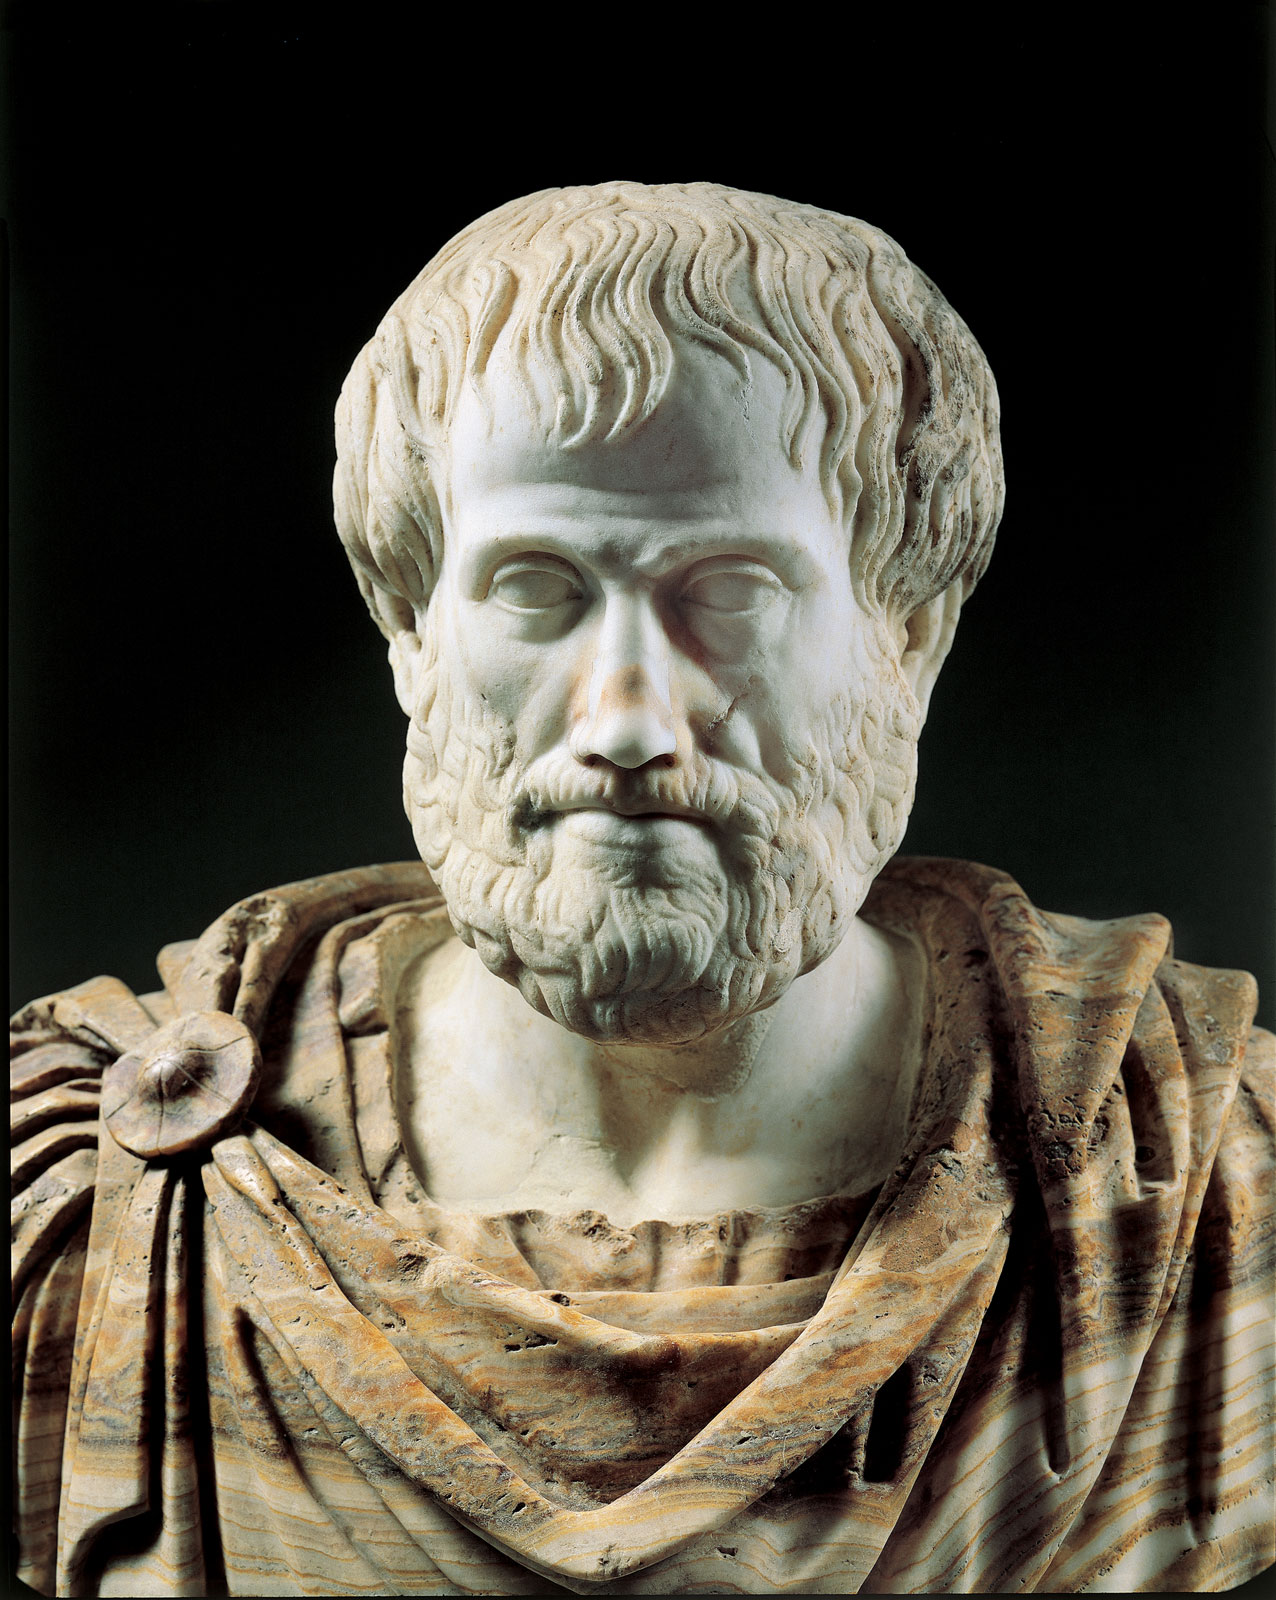
\includegraphics[height=.8\textheight]{../assets/aristotle}
    
    ``The Philosopher'' 
    \end{column}
    \begin{column}{.5\textwidth}
      \begin{itemize}[<+->]
        \item Rules of debate \& rhetoric
        \item Ancient India: Gautama, \emph{Ny\=aya S\=utras} (600 BCE-200
        CE)
        \item Ancient Greece: Aristotle (384--322 BCE)
        \item Cataloged valid arguments (``syllogisms''), e.g.,
        \item All ungulates have hooves.\\
        No fish have hooves.\\
        $\therefore$ No fish are ungulates.
      \end{itemize}
    \end{column}
  \end{columns}
\end{frame}

\begin{frame}
  \frametitle{The middle ages}
  \begin{columns}
    \begin{column}{.5\textwidth}
    
\includegraphics[height=.8\textheight]{../assets/avicenna}
    
    Avicenna! 
    \end{column}
    \begin{column}{.5\textwidth}
      \begin{itemize}[<+->]
        \item Ibn S\=\i n\=a (Avicenna) (980--1037): worked on like \textit{everything} 
        \item Pierre Abelard (1079--1142)
        %connected with conceptualism! https://en.wikipedia.org/wiki/Conceptualism
        \item William Ockham (1285--1347)
        \item Jean Buridan (1301--1358)
      \end{itemize}
    \end{column}
  \end{columns}
\end{frame}

\begin{frame}
  \frametitle{Mathematical logic}

  \begin{columns}
    \begin{column}{.5\textwidth}
    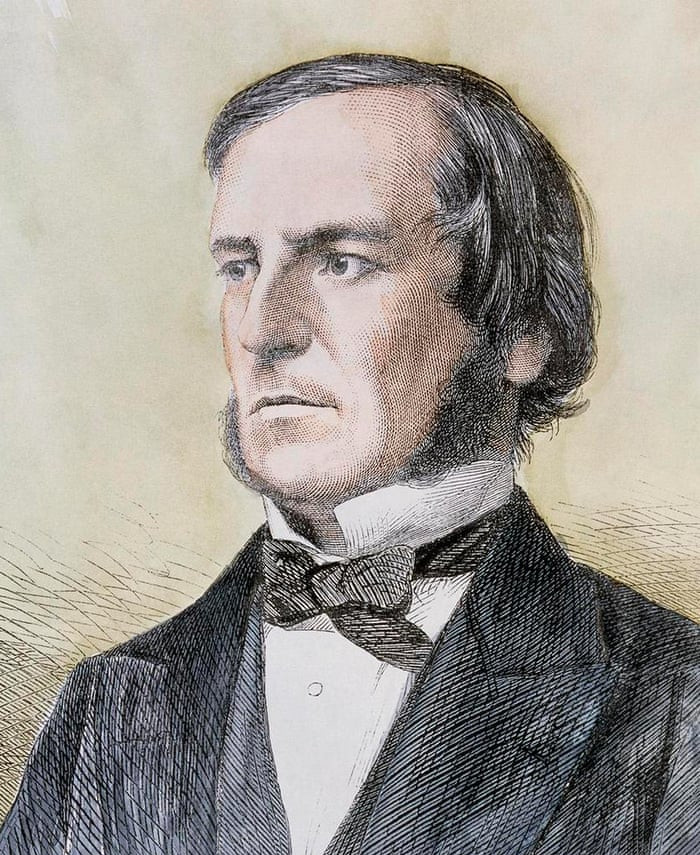
\includegraphics[height=.8\textheight]{../assets/boole}
    
    Boole! 
    \end{column}
    \begin{column}{.5\textwidth}
      \begin{itemize}[<+->]
        \item Augustus De Morgan (1806--1871)
        \item George Boole (1815--1864) [self-taught, and so can you!]
        \item Charles Lutwidge Dodgson (aka Lewis Caroll) (1832--1898) [thank him for the \emph{trees!}]
        \item John Venn (1834--1923)
      \end{itemize}
    \end{column}
  \end{columns}
\end{frame}

\begin{frame}
  \frametitle{Modern logic: Peirce at al}

  \begin{columns}
    \begin{column}{.5\textwidth}
      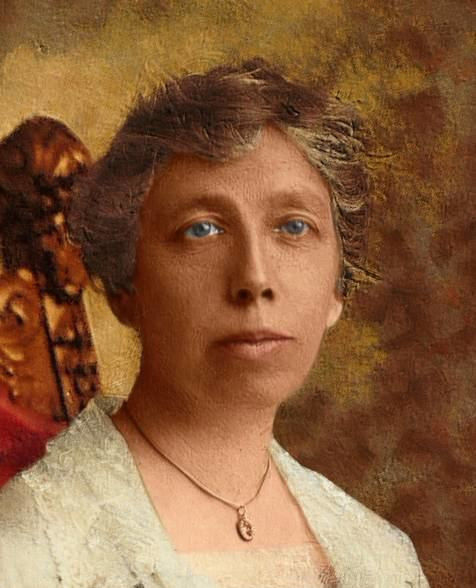
\includegraphics[height=.8\textheight]{../assets/ladd-franklin}
      
      Ladd Franklin!
    \end{column}
    \begin{column}{.5\textwidth}
      \begin{itemize}[<+->]
        \item Charles Sanders Peirce (1839--1914): a Cambridge native! 
        \item Christine Ladd Franklin (1847--1930)
        \item Ernst Schr\"oder (1841--1902)
      \end{itemize}
    \end{column}
  \end{columns}
\end{frame}

\begin{frame}
  \frametitle{Modern logic: Gottlob Frege}

  \begin{columns}
    \begin{column}{.5\textwidth}
      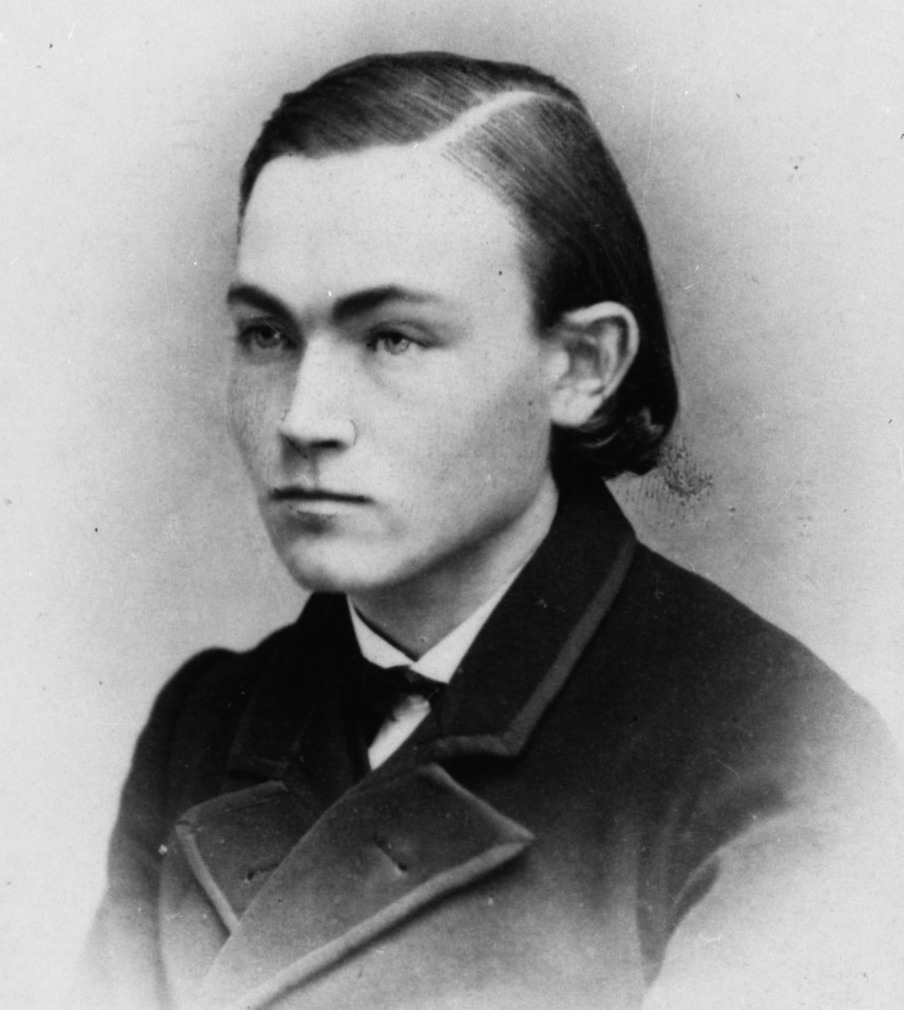
\includegraphics[height=.8\textheight]{../assets/frege}
    \end{column}
    \begin{column}{.5\textwidth}
      \begin{itemize}[<+->]
        \item 1848--1925
        \item Predicates and quantifiers
        \item Plan to turn all of math into theorems of logic alone
        \item Did \href{https://dailynous.com/2021/02/03/frege-plagiarize-stoics/}{Frege plagarize ideas from the Stoics???}
      \end{itemize}
    \end{column}
  \end{columns}
\end{frame}

\begin{frame}
  \frametitle{Modern logic: Bertrand Russell}

  \begin{columns}
    \begin{column}{.5\textwidth}
      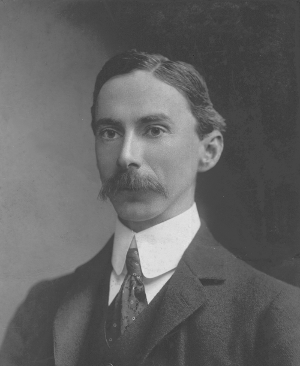
\includegraphics[height=.8\textheight]{../assets/russell}
    \end{column}
    \begin{column}{.5\textwidth}
      \begin{itemize}[<+->]
        \item 1870--1972
        \item Showed Frege's system contradictory (1902)
        \item Fixed it (\textit{Principia mathematica} 1910--13, 3 vols.)
        \item Plan to turn all of math into theorems of logic alone
      \end{itemize}
    \end{column}
  \end{columns}
\end{frame}

\begin{frame}
  \frametitle{Modern logic: David Hilbert}

  \begin{columns}
    \begin{column}{.5\textwidth}
      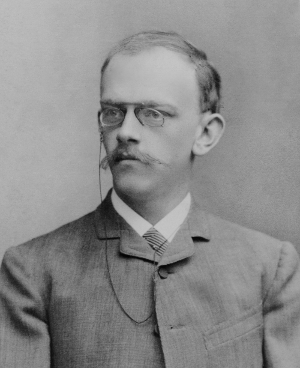
\includegraphics[height=.8\textheight]{../assets/hilbert}
    \end{column}
    \begin{column}{.5\textwidth}
      \begin{itemize}[<+->]
        \item 1862--1943
        \item Combined Russell's and Schr\"oder's systems
        \item First modern logic textbook
        \item Plan to turn all of math into consequences of a single set of premises
      \end{itemize}
    \end{column}
  \end{columns}
\end{frame}

\begin{frame}
  \frametitle{Modern logic: Kurt G\"odel}

  \begin{columns}
    \begin{column}{.5\textwidth}
      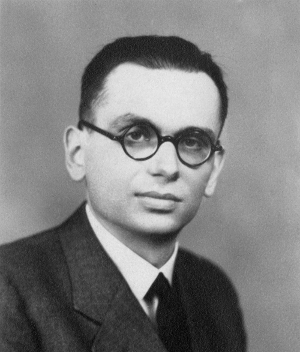
\includegraphics[height=.8\textheight]{../assets/goedel}
    \end{column}
    \begin{column}{.5\textwidth}
      \begin{itemize}[<+->]
        \item 1906--1978
        \item Showed that every valid argument has a proof
        \item Showed that Frege/Russell's and Hilbert's plans can't work
      \end{itemize}
    \end{column}
  \end{columns}
\end{frame}

\begin{frame}
  \frametitle{Modern logic: Alan Turing}

  \begin{columns}
    \begin{column}{.5\textwidth}
      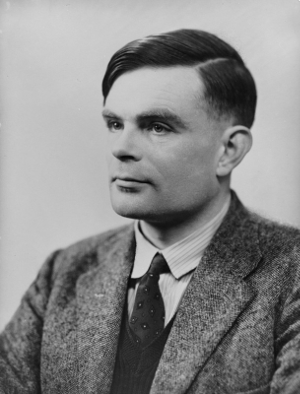
\includegraphics[height=.8\textheight]{../assets/turing}
    \end{column}
    \begin{column}{.5\textwidth}
      \begin{itemize}[<+->]
        \item 1912--1954
        \item Showed that unlike SL, QL has no decision procedure
        \item Invented Turing machines (``father of computer science'')
      \end{itemize}
    \end{column}
  \end{columns}
\end{frame}

\begin{frame}
  \frametitle{Modern logic: Gerhard Gentzen}

  \begin{columns}
    \begin{column}{.5\textwidth}
      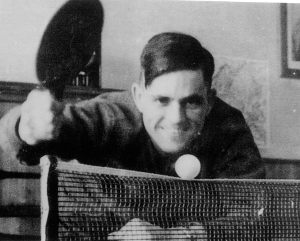
\includegraphics[width=\textwidth]{../assets/gentzen}
      
      Ping pong let's GOOOOOOO!
    \end{column}
    \begin{column}{.5\textwidth}
      \begin{itemize}[<+->]
        \item 1909--1945
        \item Invented natural deduction
        \item Founded theory of proofs
      \end{itemize}
    \end{column}
  \end{columns}
\end{frame}

\begin{frame}
  \frametitle{Modern logic: modal logic}

  \begin{columns}
    \begin{column}{.5\textwidth}
      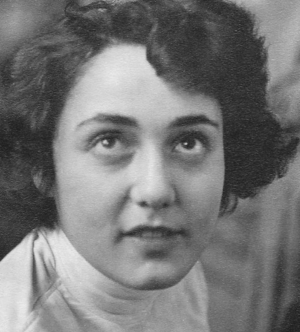
\includegraphics[height=.8\textheight]{../assets/barcan}
      
      Barcan Marcus!
    \end{column}
    \begin{column}{.5\textwidth}
      \begin{itemize}[<+->]
        \item Extend logic with operators for ``possible'' and ``necessary''
        \item Pioneered by philosophers, now used by computer scientists
        \item Rudolf Carnap, Saul Kripke, Ruth Barcan Marcus
      \end{itemize}
    \end{column}
  \end{columns}
\end{frame}




